\documentclass[../main.tex]{subfiles}


\begin{document}
\raggedright
The purpose of the project was to produce a system which will allow the students, secretary and the scrutiny panel to efficiently and securely store and access Extenuating Circumstance Forms as well as allow other staff members to access the sanitised version of the students circumstance. Django provided a simple and secure platform with the ability to access the system on any device unlike the alternates of Smart Applications and Blockchain. Smart applications would not be accessible on all devices and Blockchain would not be able to keep the data extremely confidential. Each of the following describes the requirement as well as the results achieved and why the use of Django was the right choice. 
     
\subsection*{Organised Data}
One of the issues with the previous system was the processing of data. A lot of data would be need to be duplicated which lead to unorganised data records. Students would submit multiple forms at times with either a different circumstance or the same one which would again lead to improper data storage. With the Django system the data is well organised and easily accessible. Data is stored in tables with the ability to search for specific records and view past submissions as well.  Figure \ref{fig:ecfstudenttable} and \ref{fig:ecfsectable} show extenuating circumstance forms for both Students as well as what the Secretary and Scrutiny Panel would see. The status of the form allows all stakeholders to remain informed and students avoid multiple forms filled with the same data. The search field allows sorting and filtering through the forms extremely easily when searching for students, specific forms or status search. This solves the problem of data being unorgainsed. 

\begin{figure}[H]
        \center{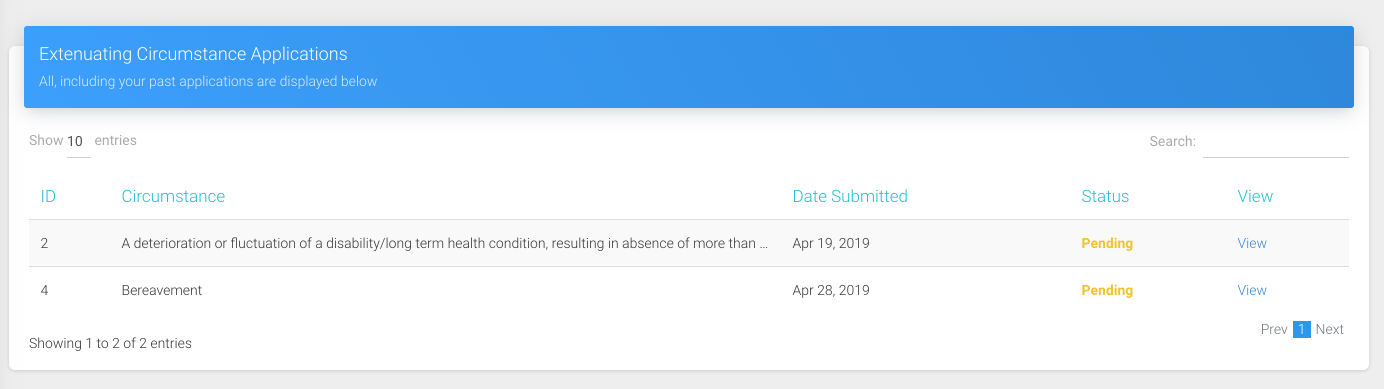
\includegraphics[scale=0.7]
        {images/ecfstudenttable.png}}
        \caption{\label{fig:ecfstudenttable} Student Panel Submitted Forms}
      \end{figure}
 
\begin{figure}[H]
        \center{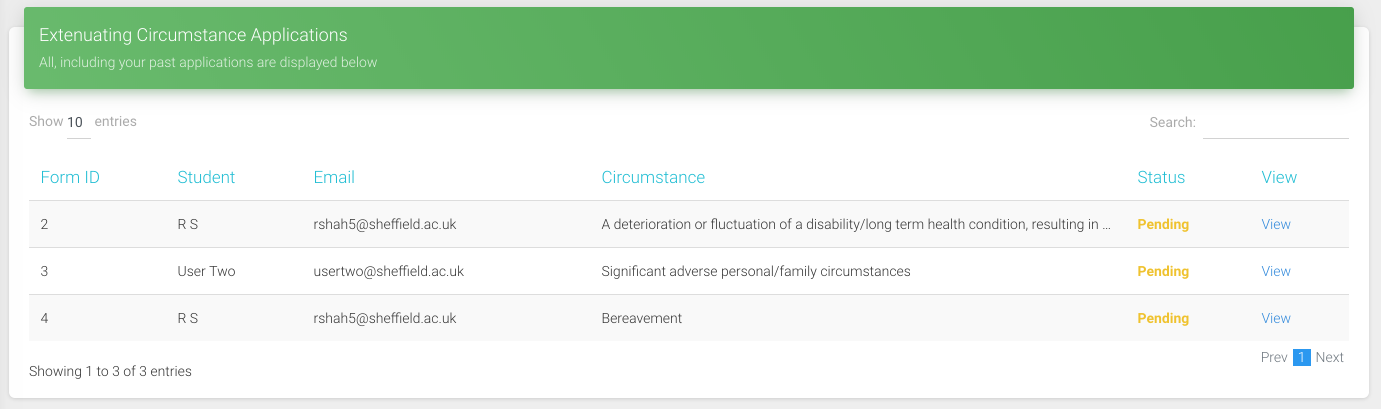
\includegraphics[scale=0.7]
        {images/ecfsectable.png}}
        \caption{\label{fig:ecfsectable} Secretary/Scrutiny Panel Submitted Forms}
      \end{figure}

\subsection*{Additional Files}
In situations where there secretary and scrutiny panel decide they need to get more proof and data from the student, the secretary can request files via the panel; automatically sending an E-mail notification to the student requesting them to submit more proof. The student can then access the form on the panel and upload the files, on successful upload another E-mail is sent to to the Secretary confirming that the student has uploaded more proof and should be taken to the next Scrutiny Panel meeting. This provides the student and the secretary simplicity as any new proof is directly linked to the form. With a web based platform like Django, using IF statements made such tasks extremely easy to code with. Figures \ref{fig:dashboardmorefiles} and \ref{fig:viewformmorefiles} show the section of additional files under the student panel. 

\begin{figure}[H]
        \center{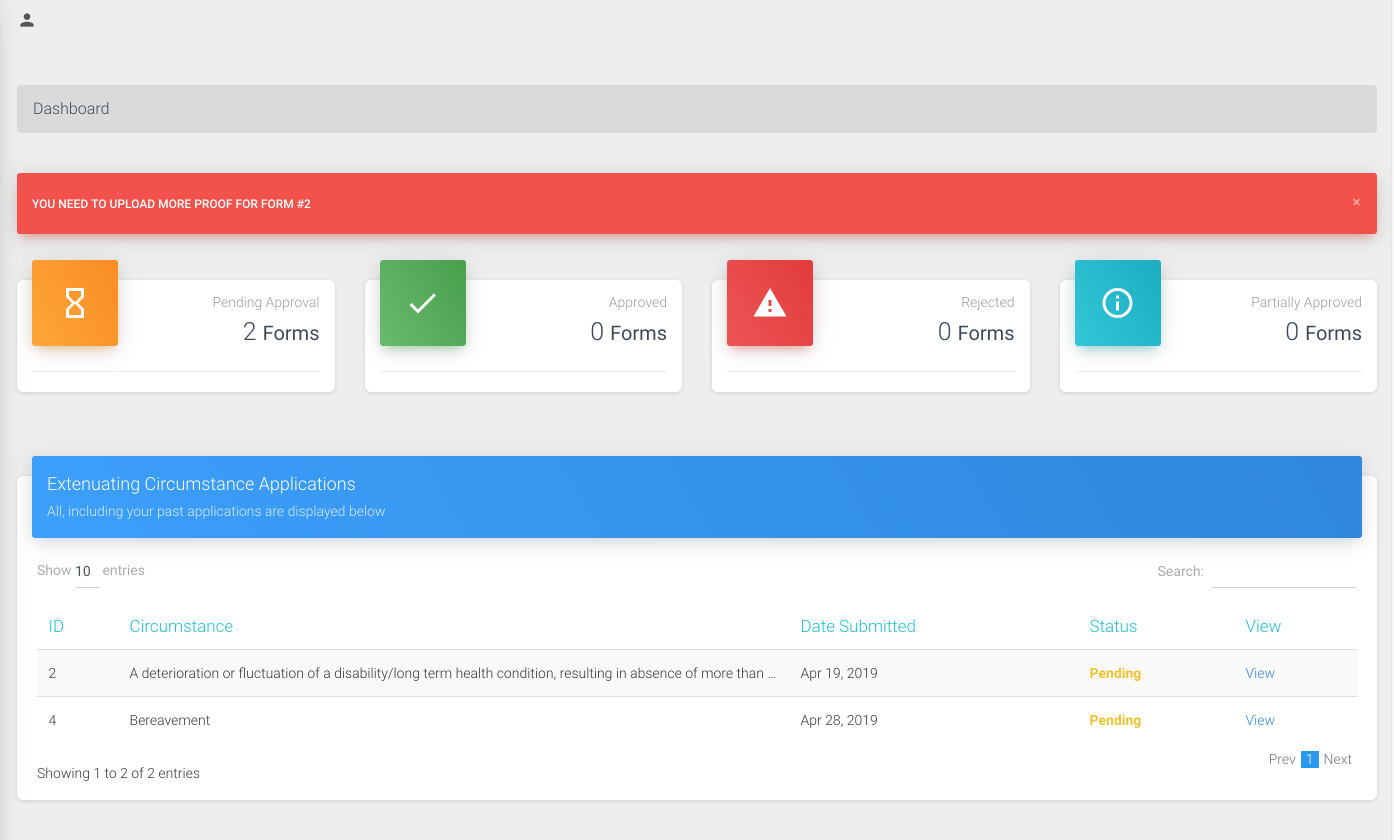
\includegraphics[scale=0.7]
        {images/dashboardmorefiles.png}}
        \caption{\label{fig:dashboardmorefiles} Dashboard notification for more files}
      \end{figure}
      
\begin{figure}[H]
        \center{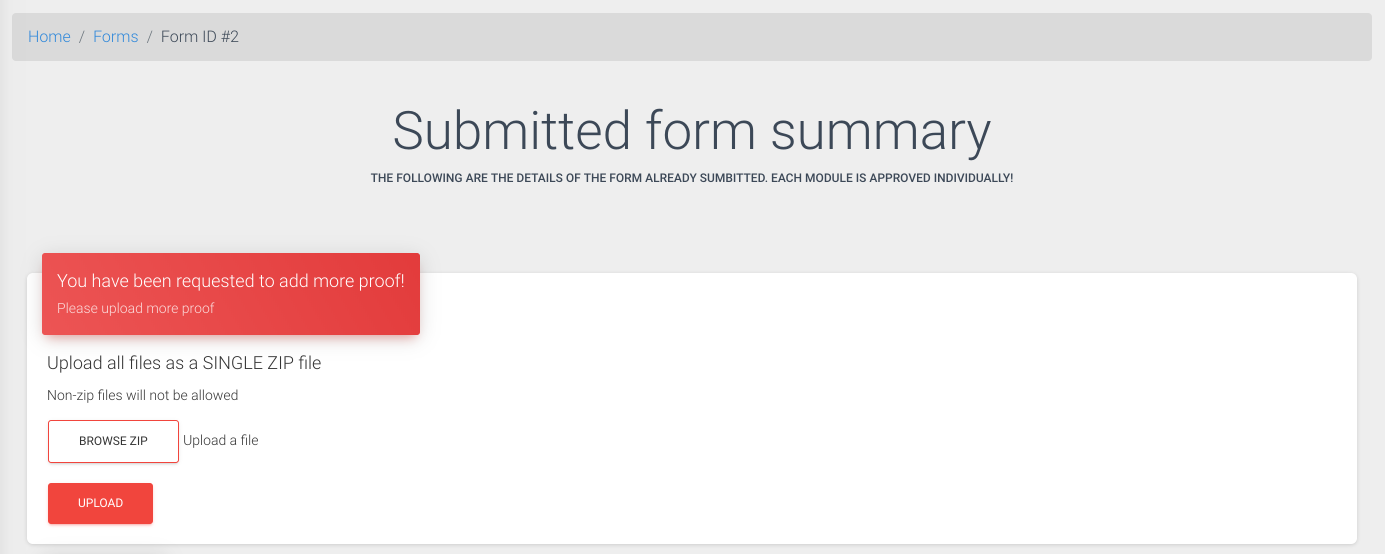
\includegraphics[scale=0.7]
        {images/viewformmorefiles.png}}
        \caption{\label{fig:viewformmorefiles} View Form upload files}
      \end{figure}
      
\subsection*{Print, Download \& Student Record}
Being able to share the data to other third parties was an important requirement as well as being able to get it on paper. With the use of JavaScript, printing and saving as a PDF document was implemented successfully with the output being exactly the same as what a user would view on the website as explained in Chapter \ref{ch:implementation}. Figure \ref{fig:print} shows two simple buttons which have the JavaScript code behind it to simply print or download the current page in the same format it is viewed. 

\begin{figure}[H]
        \center{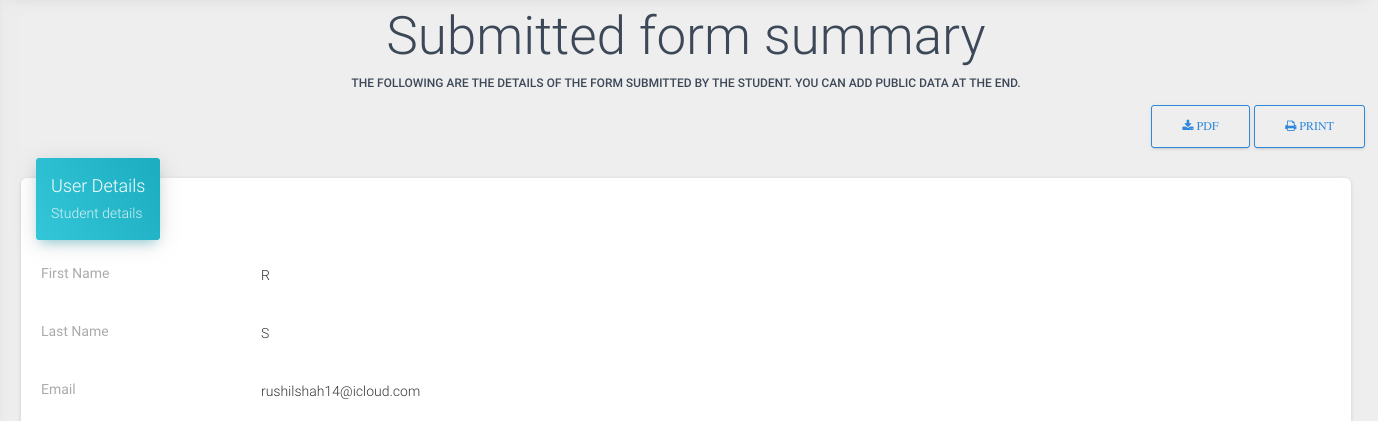
\includegraphics[scale=0.7]
        {images/print.png}}
        \caption{\label{fig:print} Print and Download Files}
      \end{figure}
      
Another requirement was being able to share the students record where the sanitised version of data is stored to the student portfolio. The current implementation uses a unique link to each students profile which can be added to the students portfolio in order to share the data. Only staff members will have access to the student portfolio hence access to the records. Figure \ref{fig:studlink} shows the secretary panel with the ability to copy the link or re-generate it to share with others. This regeneration process became extremely easy as Django uses \textit{Python} which has a \textit{random} package as mentioned under Chapter \ref{ch:implementation} allowing the link to follow a random 8 digit format.

\begin{figure}[H]
        \center{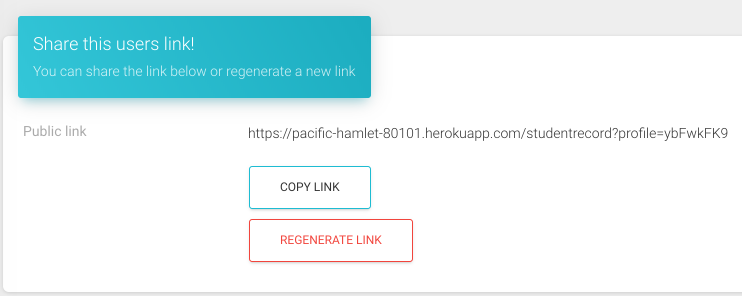
\includegraphics[scale=1]
        {images/studlink.png}}
        \caption{\label{fig:studlink} Student Record link}
      \end{figure}
      
\subsection*{Security}  
Security was one of the most important requirements for this system and with Django being the back-end controller it made the system secure. The University's login system would only work if the web based system is installed on its Intranet, for the purpose of coding the system currently uses another system. All-Auth\cite{allauth} provides validation for both logging in and sign up. It uses \textit{Bcrypt}\cite{bcrypt} encryption to securely store the password into the database. If the password is not complex enough, All-Auth would automatically bring up an error and ask the user to create a stronger password. The database itself is password protected when storing data, for example, \textit{Heroku} uses a \textit{25 digit complex password} to secure the database itself which is prevents brute-force attacks onto the database directly. The current implementation does not encrypt every single field in the database, this is in order to aviod unmaintained external code, but with the use of \textit{django-pgcrypto}\cite{dbencrypt} as a prototype each field can be encrypted making the data even more secure than it already is. \\[4mm]

Apart from the database security, it was important to make sure other users who can login to the system such as Students cannot access data which is specifically meant only for the Secretary or the Scrutiny Panel. This was successfully implemented with the use of FOR loops and IF statements as described in Chapter \ref{ch:implementation}. Django also has a controller for validation where such a function can be defined to simply check if the user has permission to access the pages. Other systems, for example R\textit{uby on Rails}, would require manual and extensive code just to ensure that the link cannot be accessed. \\[4mm]

The student record page (Sanitised version of the students circumstances) which is accessible to staff members would need to be behind \textit{University of Sheffield's Intranet} in order to authenticate if the user is a staff member or not. Even without staff authentication, the student records page can only be accessed by having the student's key as explained under Chapter \ref{ch:implementation}. A Key system would prevent unauthorised access to the students records as the link would only be accessible in the students portfolio. In cases where the link has been shared numerous times it can be regenerated by the secretary to prevent access on the old link. With access to the University's login authentication, student record would be entirely secure. However, the current system does prevent unauthorised access almost as good as the specific authentication\\[4mm]

Other security tests were also completed, some provided by Django's inbuilt tests while others required manual testing. The security requirements were satisfied based on the tests ran such as \textit{Raw SQL Queries, Cross Site request Forgery and Unittests}. However, not all code has been tested due to lack of expertise on site penetration. Experienced coders could find bugs in the code which can later be exploited if the current system is unmaintained with Django's new security updates. This issue can occur on any other system, web-based or even smart applications. Without keeping the code up to date with the latest developments in the respective language, penetration is highly possible.   \\[4mm]

Lastly, uploaded files are stored directly onto the hosting server. In order to secure the files, the use of \textit{SSH-Keys} to access the hosting server would provide increased security. Even with other web-based or smart applications the use of \textit{SSH-Keys} is extremely important as all data would need to be hosted somewhere on the cloud. Another approach, currently not implemented in the system, is to individually encrypt each file as it is stored onto the system. Two stable, but not maintained, Django encryption projects can be used. One creates a transparent layer of encryption above the files\cite{danielquinn} while the other encrypts the files based on the form input in Django\cite{ruddra}. Both provide a good level of encryption which would make all the files extremely secure and confidential. However, as they are not maintained it would be a security risk to implement them onto the current system. 

\subsection*{Mobile First}
Since the website is coded in Bootstrap 4\cite{bootstrapfour} the system follows a mobile first coding approach which allows the website to be easily accessed on any mobile devices (Smart phones, tablets or laptops) with full functionality. Students can apply for extenuating circumstances at the comfort of their home in cases where their circumstance does not allow them to move out just to submit a printed form to the office. Figure \ref{fig:mosbilesystem} shows the system running on a \textit{Heroku} Server and accessed on a mobile device as a Student trying to create a new Extenuating Circumstance Application. All panels including the Secretary Panel are mobile friendly and so can be accessed with the smallest smart phone. This is where Django turns out to be better than a simple smart application as you would need a smart phone to access the application but with Django you can access the site from any browser.

\begin{figure}[H]
        \center{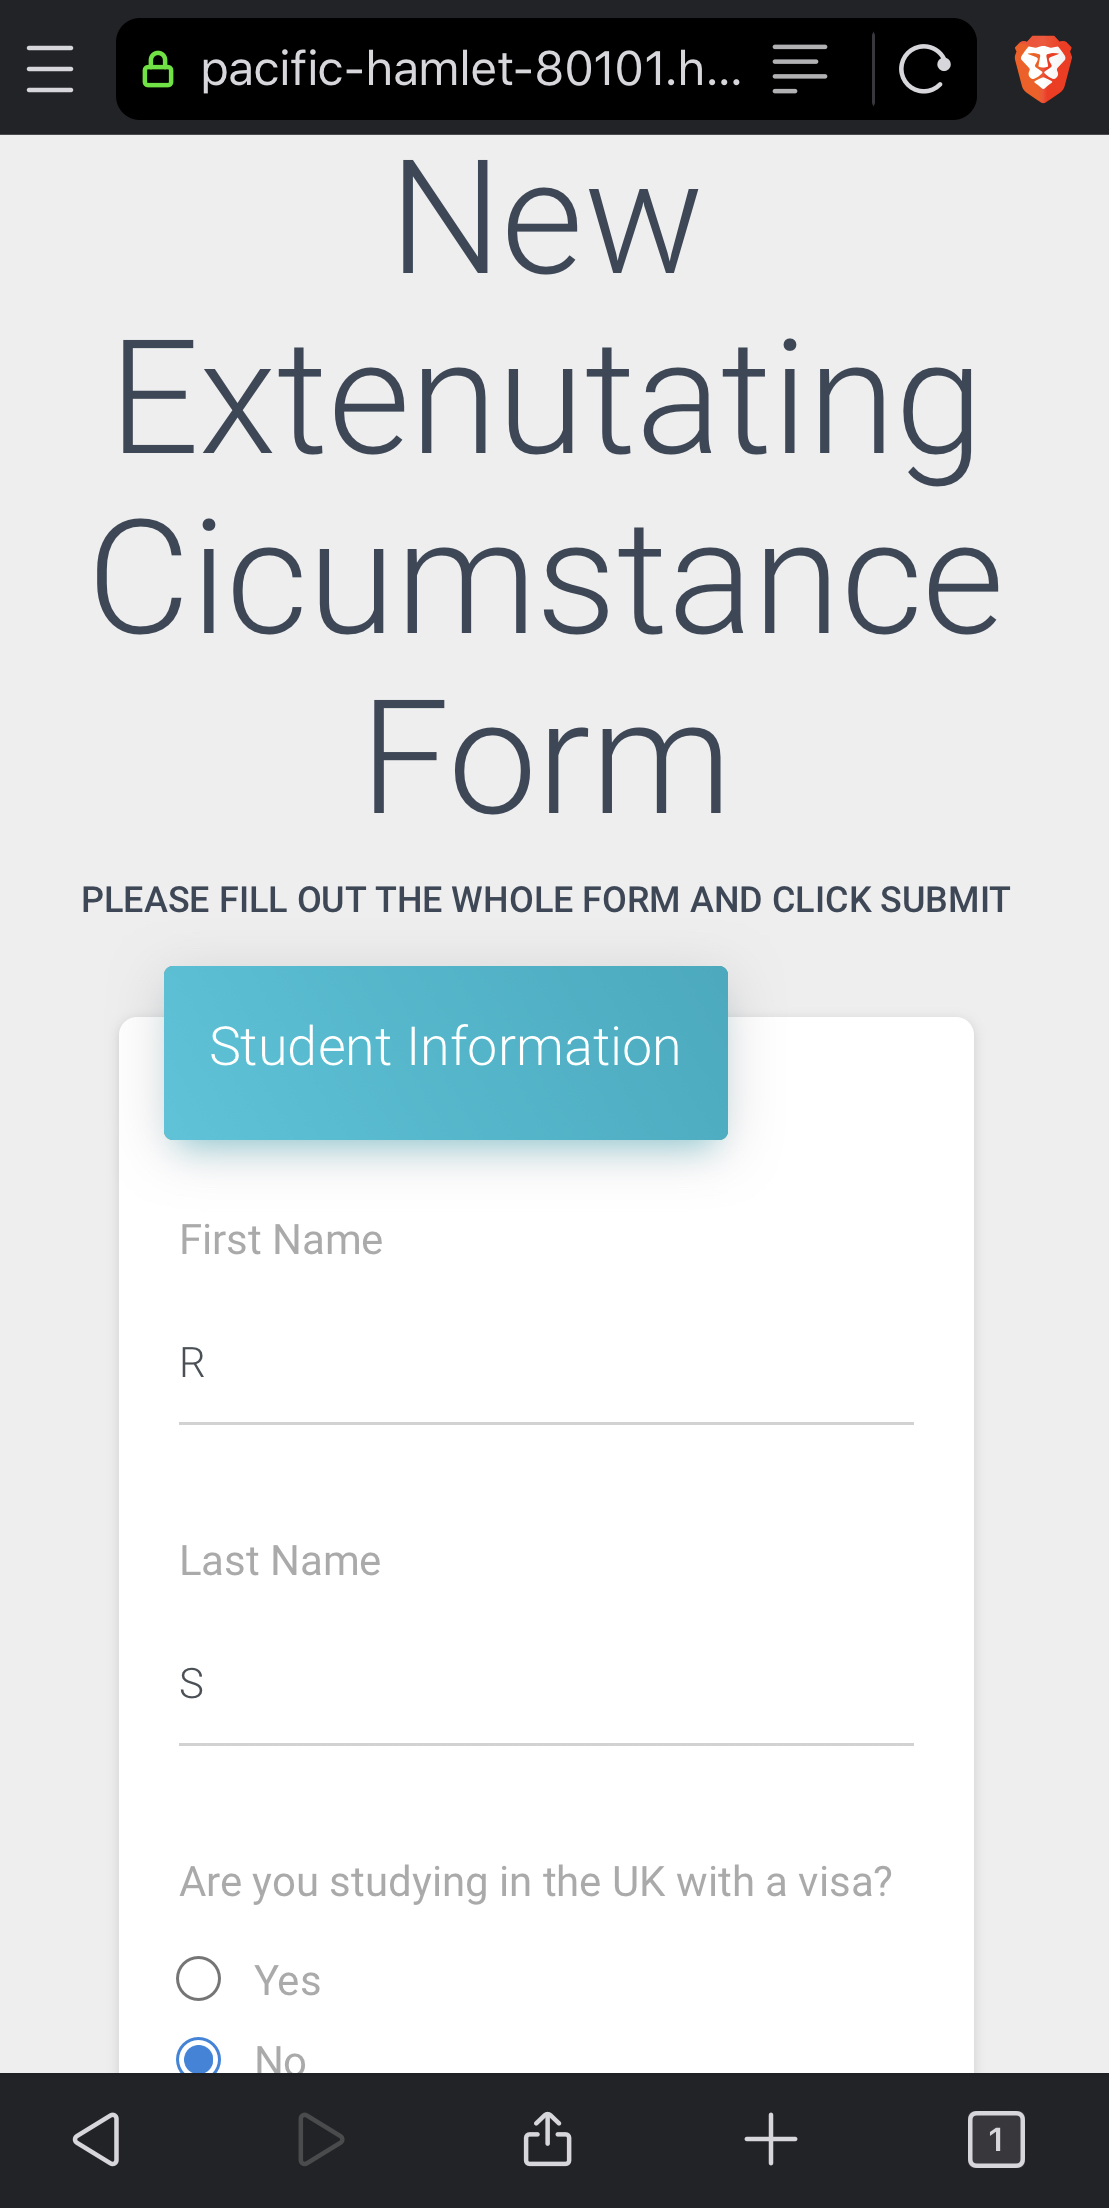
\includegraphics[scale=0.15]
        {images/mobiledevice.jpg}}
        \caption{\label{fig:mosbilesystem} Screenshot of the system running on a mobile device}
      \end{figure}

\subsubsection{Email Notifications (Additional Feature)}
Communication between the system and the users is an important feature to have. The implementation uses \textit{Django's mailer system} to send E-mails to the students as well as the secretary on successful actions such as \emph{new form submitted}. Figure \ref{fig:viewformmorefiles} showed the upload form HTML on the student panel but in order to get the attention of the student towards it, an automated E-mail is sent asking the user to submit the additional files. This is shown in Figure \ref{fig:emailuploadfiles} and \ref{fig:newformsub}

\begin{figure}[H]
        \center{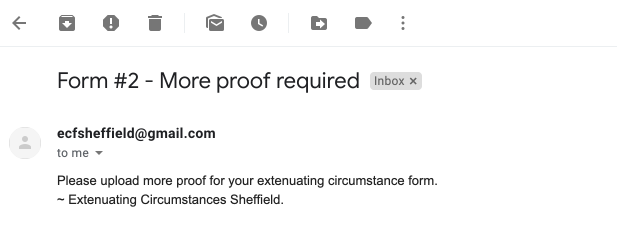
\includegraphics[scale=1.2]
        {images/emailuploadfiles.png}}
        \caption{\label{fig:emailuploadfiles} Screenshot of E-Mail received for additional files by student.}
      \end{figure}

\begin{figure}[H]
        \center{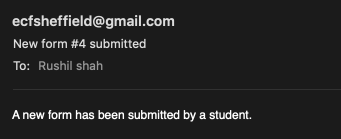
\includegraphics[scale=1.2]
        {images/newformsub.png}}
        \caption{\label{fig:newformsub} Screenshot of E-Mail received by secretary.}
      \end{figure}

\end{document}
